\newpage
\section{Constructive heuristics}

% Introduzione
\subsection{Introduzione}
Nel (caso peggiore) di variabili binarie il livello computazionale sarà dato da $O(2^n)$ quindi il tempo di calcolo cresce esponenzialmente con il numero di variabili. 

In molte applicazioni si fa affidamento ad \hl{algoritmi detti inesatti} che \hl{CERCANO di generare delle soluzioni ammissibili}. Questi rientrano negli \hl{algoritmi euristici} dove è importante che la \hl{conoscenza del progettista venga trasmessa all'algoritmo}. Questi algoritmi possono essere:

\begin{itemize}
    \item \textbf{costruttivi}: dove \hl{cercano di generare una prima soluzione ammisibile}
    \item \textbf{migliorativi}: dove \hl{prova a migliorare la prima soluzione}
\end{itemize}

Trovare una soluzione ammissibile potrebbe essere difficile dato che potrebbe essere più complicato del trovarne una ottima.


% Travellig Salesman Problem (TSP)
\subsection{Travellig Salesman Problem (TSP)}

Data una matrice $C$ di transizione dove, per andare dal punto $1$ al $2$ \hl{pago $c_{12}$} e così via per tutte le possiabili iterazioni \hl{per un numero $n$ di punti da "visitare"}. Lo scopo sarebbe trovare un circuito che tocchi tutti i punti una sola volta con \hl{costo minimo}.

Avremo che il \hl{tempo di ciclo determina la produttivita' della macchina} tipo un robot che fa n fori e conclusi gli n fori finisce oil cilo.

Un vincolo ulteriore potrebbero essere le \hl{finestre temporali} che potrebbero esserci come nei casi di consegna dei pacchi amazon, il che \hl{rende computazionalmente piu' difficile o anche inammissibile il problema}. Notare come cambiando anche solo un dato potremmo avere una soluzione ammsisibile o una crescita esposnenziale dell'infattibilità dala quele deriva l'instabilità.


% Algoritmo greedy
\subsection{Algoritmo Greedy}

Algoritmo che \hl{cerca di massimizzare nel breve periodo} (usato per essere adattato a qualsiasi problema). È un'\hl{euristica di tipo costruttivo}, infatti ha una \hl{procedura sequenziale} che costruisce la soluzione passo passo \hl{massimizzando solo l'utilizzo immediato} andando però in contro a:

\begin{itemize}
    \item una soluzione inammissibile
    \item non garantire una soluzione ottima
\end{itemize}

il suo \hl{pseudocodice} è un adattamenteo sull'algoritmo del Travellig Salesman Problem (TSP):

\begin{itemize}
    \item[] last = 1 (last = ultimo punto toccato)
    \item[] $S = \{2,3,...,n\}$
    \item[] while ($S \neq$ insieme vuoto)
    \begin{itemize}
        \item[] estrarre da $S$ un punto
        \begin{itemize}
            \item[] $i = \text{argmin}_{i \in S} c_{\text{last}, i}$
            \item[] $\text{succ}_{last} = i$
            \item[] last $= i$
        \end{itemize}
    \end{itemize}
    \item[] $\text{succ}_{last} = 1$ 
\end{itemize}

Vediamo un esempio con dati: $n = 4$ e
$$C=
\left[ {\begin{array}{cccc}
    0 & 10 & 5 & 8 \\
    10 & 0 & 2 & 1 \\
    5 & 2 & 0 & 4 \\
    8 & 1 & 4 & 0 \\
\end{array} } \right]
$$

dove applicando l'algoritmo abbiamo:

\begin{itemize}
    \item last = 1; $\rho = <2,3,4>$
    \item last = 3 ; $\rho=<2,4>$; $\text{succ}_1 = 3$
    \item last = 2; $\rho=<4>$; $\text{succ}_3 = 2$
    \item last = 4; $\rho =<>$; $\text{succ}_2 =4$
    \item $\text{succ}_4 = 1$
\end{itemize}


% Miller-Tucker-Zemlin
\subsection{Miller-Tucker-Zemlin}

Questo modello definisce delle \hl{variabili binare $x_{ij}$} per ogni coppia di punti $i$ e $j$:

$$ x_{ij} =
\begin{cases} 
    1, \text{ se } i,\ j \text{ sono/saranno visitati} \\ 
    0, \text{altrimenti}
\end{cases}
$$

avremo allora che:
$$\min \sum_{i,j} c_{i,j} x_{i,j}$$
s.t
\begin{itemize}
    \item $\sum{j} x_{ij} = 1\ \ \ \forall i$
    \item $\sum{j} x_{ji} = 1\ \ \ \forall i\ ->$ dice che ogni punto ha un suo successore
    \item $0 \leq x_{ij} \leq 1\ \ \ \forall x_{ij} \text{ integer} ->$ dice ogni punto ha un predecessore
\end{itemize}

Questi \hl{vincoli non bastano} per poter risolvere il modello, infatti non possiamo escludere di avere una \hl{soluzione disconnessa (sub-tour)}


\begin{figure}[H]
\centering
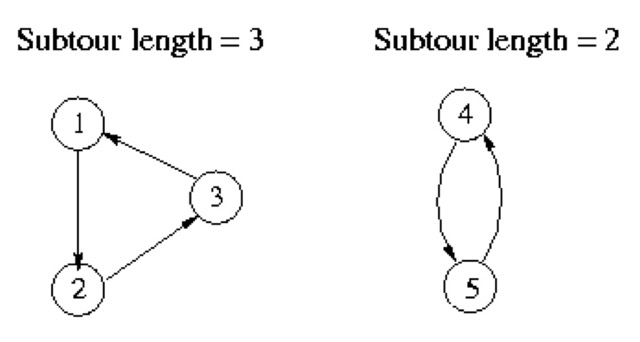
\includegraphics[scale=0.3]{sep.jpeg}
\caption{Soluzione disconnessa} 
\label{sep}
\end{figure}


Si introducono allora dei \hl{vincoli di connessione} della soluzione tramite una \hl{variabile per l'ordine di vista: $u_i$} (una per ogni punto).

Poniamo allora un punto iniziale con $u_i = 1$:

\begin{itemize}
    \item[] $u_1 = 1 -> x_{1,3} = 1$
    \item[] $u_3 = 2 -> x_{3,4} = 1$
    \item[] $u_4 = 3 -> x_{4,2} = 1$
    \item[] $u_2 = 4 -> x_{2,1} = 1$
\end{itemize}

altri \hl{vincoli da imporre su $u_i$}:

\begin{itemize}
    \item $2 \leq u_i \leq 1\ \ \ \forall i \neq 1$
    \item $u_i - u_j + 1 <= n(1-x_{ij})\ \ \ \forall i,j \neq 1$
\end{itemize}

Avremo quidni \hl{2 casi}:

\begin{itemize}
    \item $x_{ij} = 0\ \Rightarrow\ u_i - u_j +1 \leq n$: ovvio dato che tutte le variabili \textbf{$u$ sono comprese in $n$}
    \item $x_{ij} = 1\ \Rightarrow\ u_i - u_j + 1 \leq 0$: dato che $u_j \geq u_i + 1$ allora \textbf{$i$ predecessore di $j$}
\end{itemize}


% Algoritmo relax-and-fix
\subsection{Algoritmo relax-and-fix}

Si usa per \hl{problemi multiperiodali} dato che voglio poter avere un approccio con \hl{suddivisione in piu' periodi temporali}:

$$\min z = c^Tx$$
s.a.
\begin{itemize}
    \item $Ax=b$
    \item $x \geq 0$ (integer)
\end{itemize}

\hl{Partiziono le variabli in $n$ gruppi} in modo da avere variabili impiegate per un solo intervallo di tempo. Allora il problema diventa:

abbiamo alloradelle applicazioni ndove le varaibili naturalemte si dividono in gruppi datoun osviluppo temporale, il orblema allora diventa:

$$\min z = \sum_{i=1}^n c_i^Tx_i$$
s.a.
\begin{itemize}
    \item $\sum_{i=1}^na_ix_i=b$
    \item $x_i \geq 0$ (integer)
\end{itemize}

la difficoltà del problema si trova nelle molte varibili intere. Posso allora \hl{definire un problema con variaibli $x_1$ del primo gurppo intere}, per le restanti faccio un rilassamento. Potremo avere che:


\begin{itemize}
    \item ausiliario: inammissibile $\to$ iniziale: inammissibile
    \item ausiliario: sol. ottima $\to$ fisso $x_1$ alla soluzione: $x_1 = \overline{x}_1$
\end{itemize}

Quindi per \hl{risolvere il problema} dobbiamo:

\begin{enumerate}
    \item $\underline{x}_1$ diventa \textbf{intera}
    \begin{itemize}
        \item \textbf{rilasso} le altre variabili
        \item \textbf{risolvo} il problema e \textbf{fissiamo} $x_1 = \overline{x}_1$ che viene "rimossa" dal modello
    \end{itemize}

    \item ecc, ecc...
\end{enumerate}

Così facendo \hl{tengo conto delle variabili "future"} senza richiede un grande sforzo computazione, dato che lavora sul singolo gruppo.

\hl{Generallizzando}:
$$\min x = \sum_{i=1}^{k-1} c_i \overline{x}_i + c_k x_k + \sum_{i=k+1}^n c_i x+i$$
s.t

\begin{itemize}
    \item $\sum_{i=1}^{k-1} a_i \overline{x}_i + a+k x+k + \sum_{i=k+1}^n a_i x_i = b$
    \item $x_k \geq 0$ (integer)
    \item $x_i \geq 0$
\end{itemize}

Lo \hl{pseudocodice} sarà:

\begin{itemize}
    \item[] found = true
    \item[] for (k = 1 $\to$ n):
    \begin{itemize}
        \item[] solve $P_k(\overline{x}_1,...,\overline{x}_{k-1})$
        \item[] if è inammissibile:
        \begin{itemize}
            \item[] found = false
            \item[] break;
        \end{itemize}
        \item[] else: $(x'_{k+1},...,x'_n)$ è soluzione
        fissare $\overline{x}_k = x'_{k}$
    \end{itemize}
\end{itemize}


% Algoritmo rolling horizon
\subsection{Algoritmo rolling horizon}

Durante il primo periodo considero di:

\begin{enumerate}
    \item creare un \hl{sottoproblema con alcune variabili} da $x_1$ a $x_k$
    \item \hl{trascurare le variabili dei periodi successivi}
    \item fisso $x_1$
    \item mi \hl{muovo di uno step}
    \item considero un \hl{sottoproblema con $x_1$}
    \item \hl{fisso $x_2$} e considero le variabili fino a $x_k+1$.
    \item ecc, ecc...
\end{enumerate}

Andiamo quindi a \hl{risolvere un problema a $k$ variabili} ma \hl{senza tenere in conto le variabili troppo successive}, quindi sarà meno accurato.


% Multiple criteria decision making
\subsection{Multiple criteria decision making}

Spesso abbiamo \hl{piu' obbiettivi} e \hl{non riusciamo a scegliere in anticipo quale ha priorita'} allora spesso vanno in \hl{conflitto}, allora cerchiamo di trovare le migliori soluzioni che devono \hl{rispettare alcuni vincoli}:

$$p \text{ criteria } =
\begin{cases} 
    z_1 = f_1(x) \text{ da }\min \text{ o }\max \\ 
    z_2 = f_2(x) \text{ da }\min \text{ o }\max \\ 
    ... \\
    z_p = f_p(x) \text{ da }\min \text{ o }\max
\end{cases}
$$
s.t

\begin{itemize}
    \item $g(x) \geq 0$
    \item $x \geq 0$
\end{itemize}


% Esempio problema scheduling
\subsection{Esempio problema scheduling}

Preso un problema di scheduling, abbiamo $n$ attività con paramentri:

\begin{itemize}
    \item $S_i$: starting time dell'attività $i$
    \item $d_i$: durata dell'attività $i$
    \item $p_{ij} = 1$ se l'attivtà $j$ è prerequinistito dell'attività $i$
    \item $p_{ij} = 0$ altrimenti
\end{itemize}

come f.o: $\min T$ con $T$ tempo di completamento:
$$\min T$$
s.t.

\begin{itemize}
    \item $T \geq S_i + d_i,\ i = 1, ..., n$
    \item $S_i \geq p_{ij} (S_j + d_j),\ i,j = 1, ..., n$
\end{itemize}

Per poter \hl{formulare un'attivita' in modo fattibile}:

\begin{itemize}
    \item $D_i$: max durata dell'attività $i$
    \item $b_i$: min durata dell'attività $i$
    \item $d_i$: durata dell'attività $i$
    \item $X_i$: costo per accellerare il completamento dell'attività $i$
\end{itemize}


allora:

\begin{itemize}
    \item $d_i = D_i-a_iX_i$ con $a_i$ coefficente in unità di tempo
    \item $d_i \geq b_i$
\end{itemize}

abbiamo da minimizzare 2 obiettivi:
$$min \sum_{i=1}^n X_i$$
$$min T$$
s.t.

\begin{itemize}
    \item $T \geq S_i + d_i\ \ \ \forall\ \ \ i$
    \item $S_i \geq p_{ij} (S_j + d_j)\ \ \ \forall\ \ \ i, j, i \neq j$
    \item $d_i \geq b_i\ \ \ \forall\ \ \ i$
    \item $d_i = D_i - a_i X_i\ \ \ \forall\ \ \ i$
\end{itemize}


% Superior solutions
\subsection{Superior solutions}

Preson un problema con \hl{piu' obiettivi} allora ne consideriamo uno con obiettivo singolo, allora \hl{rappresento i singoli obiettivi} nello spazio.

Presa una soluzione potremo trovarne una migliore ma solo \hl{se si trova nella zona ammissibile e che sia nella frontiera}, in caso contrario è detta \hl{utopia}.

\begin{figure}[H]
\centering
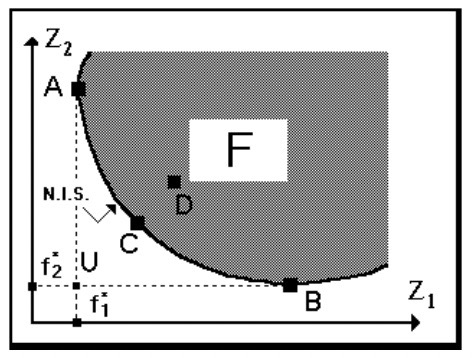
\includegraphics[scale=0.3]{utop.jpeg}
\caption{Utopia} 
\label{utop}
\end{figure}

Definiamo invece \hl{soluzione superiore} la soluzione che minimizza o massimizza meglio di tutte (come U se fosse nella zona ammissibile).

Si parla allora di soluzioni dominate e soluzioni non dominate (di \hl{Pareto}).

Per \hl{confrontare due soluzioni di Pareto} usiamo il \hl{trade-off ratio} tamite:

$$|\frac{z_i(x_A)-z_i(x_B)}{z_j(x_A)-z_j(x_B)}|$$

che rappresenta il \hl{miglioramento dell'obiettivo i-esimo in base al miglioramento di un altro obiettivo}.

Nel caso di una \hl{zona convessa} collegneremo i punti limite tramite una \hl{tangente immagginaria}, dalla quale però non prendere mo i punti di frontiera.

\begin{figure}[H]
\centering
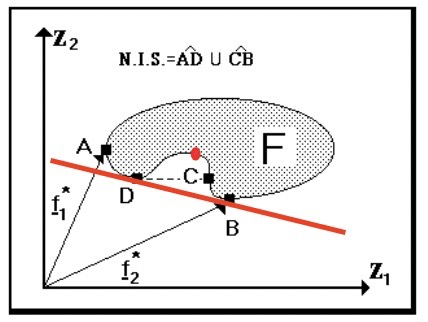
\includegraphics[scale=0.3]{convess.jpeg}
\caption{Zona convessa} 
\label{convess}
\end{figure}

per \hl{trovare le soluzioni efficenti} abbiamo 2 metodi:

\begin{enumerate}
    \item \hl{metodo dei vincoli}: \textbf{considero un solo obiettivo}, per gli altri avrò:
        $$\min f_i(x)$$
        
        s.t
        
        \begin{itemize}
            \item $f_k(x) \leq u_k$
            \item $g(x) \geq 0$
            \item $x \geq 0$
        \end{itemize}

        Prendo allora solo $A$ e $D$:

        \begin{figure}[H]
        \centering
        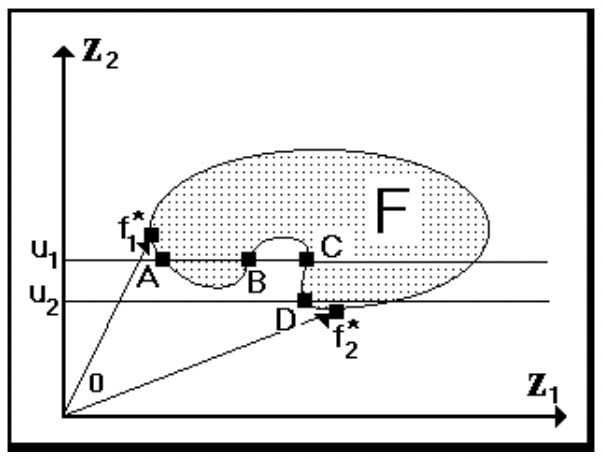
\includegraphics[scale=0.3]{vinc.jpeg}
        \caption{Metodo dei vincoli} 
        \label{vinc}
        \end{figure} 
    \item \hl{metodo dei pesi}: abbiamo una sola \textbf{f.o somma di tutti li obiettivi}:
        $$\min \sum_{i=1}^p w_i f_i (x)$$

        s.t
        
        \begin{itemize}
            \item $\sum_{i=1}^p w_i = 1$
            \item $g(x) \geq 0$
            \item $x \geq 0$
            \item $w_i \geq 0$
        \end{itemize}

        \begin{figure}[H]
        \centering
        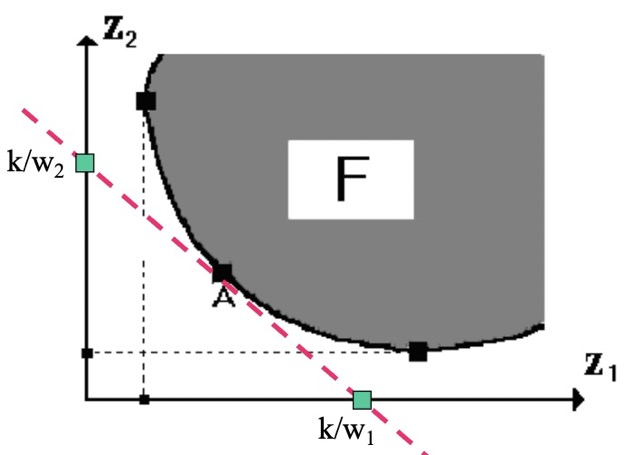
\includegraphics[scale=0.3]{pesi.jpeg}
        \caption{Metodo dei pesi} 
        \label{pesi}
        \end{figure}

        dove a seconda del valore che diamo ai pesi andiamo a \hl{spostare la retta trangente alla zona ammissibile}.
\end{enumerate}


% Metodo a priori
\subsection{Metodo a priori}

Per \hl{risolvere il singolo problema} usiamo:
$$\max U(f_1(x), f_2(x), ..., f_p(x))$$

s.t
\begin{itemize}
    \item $g(x) \geq 0$
    \item $x \geq 0$
\end{itemize}

ma in genere \hl{non si trova} questa soluzione.


% Metodo a posteriori
\subsection{Metodo a posteriori}

Generiamo tutte le \hl{soluzioni efficienti per dire quale e' la migliore}. Notare che così facendo si potrebbe avere una \hl{crescita esponenziale} del problema.

Una buona \hl{alternativa} è il metodo interattivo.


% Metodo interattivo
\subsection{Metodo interattivo}

Presi 2 obiettivi:

\begin{itemize}
    \item troviamo il \hl{punto ottimo per entrambi}
    \item troviamo la \hl{prima soluzione efficiente che sia tra $A$ e $C$}
    \item scegliere su \hl{quale parte della frontiera posizionarsi}
    \item ecc, ecc...
\end{itemize}

\begin{figure}[H]
\centering
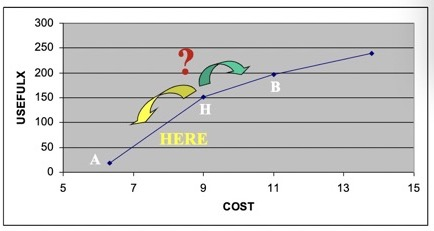
\includegraphics[scale=0.5]{intent.jpeg}
\caption{Metodo interattivo} 
\label{intent}
\end{figure}

mi fermerò quando il segmento che rimane è \hl{cosi piccolo che i due punti conincidono}.









LOCAL SEARCH:
algoritmo di tipo euristico migliorativo, cioe1 presuppone che sia stata gia prodotta una soluiozne ammissibile. 

diviimao le procedure in:
singola produzione: migliorear in un intorno la situazione (in modo locale) in genre rimane bloccata in minimi locali. l'algoritmo parte da una soluizone iniziale e megliorandola cercara sempre di genrare una successione di soluzione ammissibili

multiple population: ad ogni iterrazione hanno una popolazione di soluzioni, quidni non ne hanno solo una

non sono algoritmi precisi ma bavnno poi adattati al particolare proboema che si intende affrontare

progeto di ricerca locale: si parte da un asoluzione corrente  $x^{(0)}$. l'intorno di x0 (N(xo) e1 un insieme di soluzioni vicine ad x0 dove la definizione viene data dal progettista. solo nell'intorno dei viscinin possiamo trovare la soluizone. trovaimo allora la soluzione in N(x0) allora aggiungiamo un vincolo:
$$\unerdline{x} \in N(\underline{x}^{(0(})$$

osi trovo la coluzione x1.

questo apposccio puo1 esere ripetuto per ogni soluizone che trovo.

cosi avremo un algoritmo di discesa/ascesa se stiamo min/max.

img finche non ci sono piu soluzioni migliorative nellasoluzione corrente quidni la'lgoritmo rimane bloccato in un ottimo locale, cioe quello del proprio intorno
in genere un probelma non convesso posso avere un ottimo locale di scarsa qualita nel contrario puo1 essere uguale a quello globale.

pseudocodice:
...


sono questi problemidi tipo euristico allora per poterlo implementare devo specificare un intorno che tenga ocont delle peculiarita di un problem

es1: problemsa del tsp
una soluzione e1 una permutazione del numero di punti. per definire un introno su una situazione del tipo:

img

dobbiamo definire una perturbazione della soluzioene cancellando 2 archi della soluzione es: x13, x25 allora avremo un asoluzione disconnessa 16742 e 35. posso fare una giunzione tra i due segmenti aggiungendo x15 e x23 si dice allora approcci odistroy and repear. quindi vado a mettere in dubbio dei collegamenti e poi cerco di trovare una soluzione piu efficente. potrei allora avere una variaczione di csoto: 
$$\Delta z = c15 + c23 = c13 = c25$$
cioe archi che ho aggiunto meno quelli tolti.

cambiare x52 non x25

questa e1 un single move. in intorno e1 un inseme di tutte le soluzioni che si ottengon ocancelando 2 archi e riaprandoli. un intorno e1 definito come insieme di tutte le soluzioni ch esi possono ottenre con il delete and repear quindi cancello 2 archi non contiguie poi recupero l'ammissibilita con il repear.

la miglior perturbazione e1 la suoluzione successiva.
se delta z = 0 ci fermiamo localmente 

approcci o3 opt cancello 3 archi alla volta e ricorstruisco 

nel 2 opt avremo n^2 vicini





LOCAL BRANCHING:
avendo u nproblema a grandi dimensioni con variabili binarie x1, ..., \in <0, 1> possiamo alora definire un intorno di un aoluzione. se vogliaomo usare un solver dobbiao esprimere il vincolo sottofrma di dis/equanzione lineare (vincolo: x \in N(xk)). per poterlo fare usiamo la distanza di hamming dove date 2 stringhe binarie. confronto alllora i biti omologhi e conot il numero di bit diversi:

es:...

per definire l'introno diciamo: data una soluizone corrente xk allora una soluzione x \in N(xk) se per definizonie la distanza di hamming tra x e xk e1 <= ad un valore m "
$$$$

dove se m = 10 indica di trovare le soluiozi che distano nemo di 10 bits

allora scrivo in vincolo della distanza di hamming come disequazione lineare:
$$\sum_{\forall j =1, .., n: x_j^(k) = 0} x_j + \sum ...$$

in modo da farci dare dei contributi solo se il valore e1 diverso scrivamo per una sequenza: \undreline{x}k = (0, 1, 1, 0, 1, 1) allora la disequazione lineare sara1:
$$x_1 + (1-x_2) + (1-x_3) + x_4 + (1-x_5) + (1-x_6) \leq 3$$









MULTIPERIOD LOT SIZING MODEL:
andiamo a discretizare il tempo e quidni divido la pianificazione in slot di tempo esistenti come ore sttimane mesi. avremo allora una deomanda d_t che fa tioferimenteo al periodo t che e1 un intero t = 1, .., T con Tlunghezza dell'orizzonte di pianificazione.

img

avro dei costi fissi di produzione f_t che potrebbe dipendere dal periodo dato che alcune risorse potrebbero essere piu costose in certi punti e meno in altri es: gas (non dipendon odalla uqntita prodotta)
costi variabili c_t: costi per produrre un prodotto che potrebbe dipendere dal periodo t su periodi temporali lunghi es: vegetali
costi di stockaggio h_t usata per tenere a scorta u nprodotto per un tempo t
capacota di magazzino: Q
]
variabli decisionali:
variabili di accenzione: y_t variaibli binaria 0, q acceso, spento (se produco)
var buone: essendo continnue danno meno problemi:
x_t quanto produzioamo nel periodo t. in genre imi conviene anticipare la fdoana per non pagare i costi fissi troppe volte (quanto produco)
I_t livello delle scorte alla fine del periodo t


funzione obiettivo:
somma dei costi fissi di produzione e variabili di produzione e di inventario:
$$z = \sum ...$$


vincoli di conservazione della materia: (va scritto per ogni periodo)
pe rogni periodo t il livelo delle scorte fino al perioodo precedente + cioe che ho pordotto ora - cioe che ho dato al mercato = livello delle scorte alla fine del periodo:


vincolo di capacita:
livello delle scorte non deve superare la capita di magazzino:


vincolo che lega le varaibili y a quelle x cioe accezione e spegniemnto con quntita produttiva:
$$x_t \leq \sum ...$$

dato che yt e1 binaria se: 
= 1: x_t \leq \sum ... quindi la la quantita che abiamo adesso non deve superare quello che ci viene richiesto successivamente cioe che non posso escludere che in questo periodo t produca tutto il fabisogno che seguira1
= 0: xt \leq 0, xt = 0: se non accendo gli impianti non posso produrre nulla


vincoli sull'inventario:
I_0 = 0
I_T = 0





VARIANTE BEER GAME:
1. nel problema reale non sono certo di soddisfare al domanda. potrebbe succeder di andare sotto scorta per cercare di soddisfare la domanda allora quento comporat un costo, allora il livello dele scorte si divide in un aprte positiva ed una negativa:  se finisco sotto scorta = se i+>= 0 abbiamo delle unita in inventario, oppure i- >= 0 abbiamo un arretrato ed andiamo sottoscorta

funzione obiettivo:
$$z = ...$$

vincolo di conservaione della materia sostituiamo I_t con + e -:
$$..$$

vinclo di capacita:
I_t+ \leq Q


2. riotardo dell'arrivo degli orfdini: durante le prime l settimate non posso sperare di ricevere rifornimenti per come e1 scritto il problema avremo che xt e1 la quntita che odiniamo nel periodo t e che arriva nel periodo t+l
$$...$$

potrei finire sottoscorta nel primo periodo, avremo allora che all'istante t ricevo cio che ho ridinato all;istnte t-l
$$..$$















PROBLEMI DI FLUSSO SU RETI (NETWORK FLOW PROBLEMS)
dove abbimao un grafo  con dei sui parametri che assieme formano un network. dobbiamo allora capire con=me un flusso di dati transitra nellarete.
primo porblema che vediamo
PROBLEMA DI FLUSSO A COSTO MINIMO:

ha la varainte lineare
variante single commodity


in questa classe di problemi abbiamo un grafo G(V, A)
con v vertici e A archi

img


inq uestso caso ogni vetice $i \in V$ o generea o assorbe un flusso di materiali, dati, ecc...

parametro per i nodi:
questo $\forall i \in V: d_i$
> 0 per i = sorgente (souce)
= 0 per i = transito
< 0 per i = pozzo (sink)


se d_i > 0 indica un afornitura
< 0 indica una domanda

caristiche:
single commodity: flusso omogeneo
multiple comodity: varie tipologie di flusso 


parametri per gli archi
prendo un parametro c_{ij} cioe un arco che colega i nodi i e j. c_{ij} = costo (di traspost) unitario (per unita di flusso)
altro paramentro q_{ij}: capacita massima (qunato flusso puo transitrar da i a j)


decisione da prendere: allocaizone del flusso, cioe qunto flusso deve transitare su ogni arco
le varaibili saranno: x_{ij} >= 0 fluso che transita da i a j per unita di tempo


affinche si possa avere una soluzione ammissibile una condizione necessaria e1 che se sommiamo su utti i vertici le quntita d_i devo avere 0:
$$\sum_{i\in V} d_i = 0$$

quindi non sara sufficiente per via delle capacita degli archi



misure di prestazione della f.o.:
vigliamo allora minimizzare il costo totale di trasporto su tutti gli archi:
$$\min \sum_{(i,j)\in A} c_{ij} x_{ij}$$

notaione epr definire un insieme di vincoli:
dato uun nodo i al quale abbiamo archi uscenti ed entranti allora tutti li archi entranti associamo un insieme $\delta^-(i)$ per quellio uscenti: $\delta^+(i)$


definiiamo allora i vincoli, dobbiamo tenere in conto dei vincoli di conservazione del flusso: cioe che dtutto quello cheentra nel nodo deve uscirci:
$$\sum_{(i,j)\in\delta^+(i)} x_{ij} - \sum_{(j,i)\in\delta^-(i)} x_{ji} = d_i\ \ \ \forall\ \ \ i\in V$$

altri vincoli per avere una soluzione ammissibile abbiamo ance dei vincoli di capacita: avremo un vincolo associato ad ogni arco:
$$x_{ij} \leq q_{ij}\ \  \forall\ \ \ i,j\in A$$

vincoli di non negativita:
$$x_{ij} \geq 0 (\geq l_i)\ \ \ \forall\ \ \ i,j\in A$$

dove l_i quantita minimia in caso di evenienza

la formulazione compatta dice:
$$\min z=\sum_{(i,j)\in A} c_{ij} x_{ij}$$
s.t
- $\sum_{(i,j)\in\delta^+(i)} x_{ij} - \sum_{(j,i)\in\delta^-(i)} x_{ji} = d_i\ \ \ \forall\ \ \ i\in V$
- $x_{ij} \leq q_{ij}\ \  \forall\ \ \ i,j\in A$
- $x_{ij} \geq 0 (\geq l_i)\ \ \ \forall\ \ \ i,j\in A$

formulaizone estesa:
in una topologia di rete cone questa:

img

ad ognmi arco indico c_ij e q_ij e per ogni nodo d_i

allora la fomulazione estesa e1: (prendendo il parametro del costo)
$$\min z = 2x_{12} + 5x_{13} + 3x_{23} +3x_{24} + 3_{x32} + 4x_34} + 3x_{42}
s.t
per i = 1: $x_{12} + x_{13} = 10$
per i = 2: $x_23 + x_{24} - x_{12} - x_{42} - x_{32} = 0$
per i = 3: $x_{32} +x_{34} - x_{13} - x_{23} = -3$
per i = 4: $x_42} - x_{24} - x_{34} = -7$

guardando la capacita scriviamo anche:
$x_{12} \leq 8$
$x_{13} \leq 2$
$x_{23} \leq 4$
$x_{24} \leq 7$
$x_{32} \leq 4$
$x_{34} \leq 5$
$x_{42} \leq 7$

$x_{12}, $x_{13}, x_{23}, x_{24}, x_{32}, x_{34}, x_{42} \geq 0$



se un instanza del problema e1 ammissiibile, cioe se lo sono i dati del problema, allora:
- puo esistere una soluzione ottima
- puo esere unbounded se esiste qualeche arco (i, j) \in A con costo negatico c_{ij} < 0

img

poiche il costo totale negativo nel loop 2,4,5 allora abbiamo:
$$x_{12} = 1, x_{23} = 1, x_{24} = x_{45} = x_{52} = + \infty$$

siuponendo capacita infinita

importante condiione e1 quella di interezza: dice che se i dati d_i e le capacita q_{ij} sono interi, allora esiste una soluizone ottima non unbounded che e1 anche esse interacioe x_{ij \in N_0}, cioe i flussi ottimali sono interi.


abbiamo dei casi speciali del problema di flusso a socoto minimo:
- problem a di trasprto (rtansportation problem)
- prob di assegnamento (assignment problem)
- problema di cammino piu breve/rapido (shortesr/quickest path)
- problema di massimo flusso (aximum flow problem)




PROBLEMA DI TRASPORTO:
consideriamo la variante di simple commodity( supponiamo di avere un grafo diaprtito dove l'insieme dei vertici e1 composto da due insiemi disgiunti: sorgenti (fino a m) e pozzi (fino a n). ad ogni soegente e1 associata un s_1, .., s_m \geq 0 che definiscono la fornitura e ai pozzi invece abbiamo una qunatita b_1, ..., b_m che rappresenta la domanda. tra questi vertici nei due insiemi abbiamo na coppia di sorgente-pozzo e per ogni arco ij e1 associato un costo cij (costo i trasporto per unita di flusso)

img

allora il grafo G e1 dato da: G = (V=v_1 \cup V_2, A) con V_1 \cap V_2 = insieme vuoto e viene detto grafo rbipartito ed e1 questo problemaun caso speciale del problema di flusso a caso minimo, nel qule abbiamo che:
- non abbiamo vincoli di capacita
- non abbiamo nodi di transito

il problema sara allora ammissiible se:
$$\sum_{i\in V_1} s_i = \sum_{i\in V_2} b_i$$

allora le varaibili abbiamo che:
$$x_{ij}, i\inV_1, j\in V_2$$ che indica qunate unuta di flusso ("merce") vengono gtraspostate da i a j


l'obiettivo e1 minimizzare al f.o. quindi la misura di prestazione sara: $\min z = \sum_{(i,j)\in A}\sum_{j\inV_2} c_{ij}x_{ij}$ alora minimizziamko il costo totale.

vincoli:
$$\sum_{j\in V_2} x_{ij} = s_i\ \ \ \forall\ \ \ i\in V_1$$ per ongi vertice sorgente
$$\sum_{i\in V_1} x_{ij} = b_i\ \  \\forall\ \ \ j\in V_2$$ per ongi vertice pozzo
$$x_{ij} \geq 0\ \ \ \forall\ \ \ i\in V_1, j\in v_2$$



PROBLEMA DI ASSEGNAMENTO LINAERE:
abbiamo sempre un siseme di vertici diviso in due grupi: n risorse e n tasks
obiettvo assengare le risorse ai tasks

img

assegnamo iun costo sll'arco ij con c_{ij}.

ad una risorsa possiamo associare un solo task.
es: magazzini (impianti) automatizzati: n = 4 con n risorse = ABV (automated guided vehicle)
abbiamo dei task da compiere come lo spostamente di un veicolo da un punto ad un altro

img

avremo allora i costi di oni veicolo per spostarsi allinizio del task
costi = tempo di viaggio dal puno di prelievo al punto di inizio

quindi questa tipologi a di problemi e1 un acso speciale del prtiblema di trasposto dove cambia solo che:
- m= n
- s_i = 1 \forall i
- b_i = 1 \forall j


le variabili saranno allora:
x_{ij} = 1 se la rosorsa i e1 aasegnata ad un task j
= 0 altrimenti

vorremo allora minimizzare la f.o.: $\min z = \sum_{i=1}^n\sum_{j=1}^n c_{ij} x_{ij}$
s.t.
- $\sum_{j=1}^n x_{ij} = 1\ \ \ \forall\ \ \i=1,...,n$ cioe ogni risrosa deve essere assegna ad un solo task
- $\sun_{i=1}^n x_{ij} = 1\ \ \ \forall\ \ \ j=1,...,n$ cioe ongi task deve essere assegnato ad una sola risorsa

dato che s_i = 1 con i = 1,...,n e b_j = 1 con j=1,...,n

possiamo imporre che x_{ij} \geq 0 impedendo che la variabile sia <= 0 qusto grazie all;interezza dei dati e ai vincoli qui sopra che impediscono che le varaibili assumano valore > 1 quidni potremo avere con valore 0 o 1.










